
\chapter{Results}
\label{ch:results}

Results are organised by hypothesis, not by experiment. Each section states the
question, the measurement, and the verdict.

\section{Two cohorts, and why they are labelled}

Two sets of models appear in this chapter and their field numbers differ. They are
not contradictory and they are not interchangeable.

\begin{table}[H]
\centering
\caption{The two model cohorts used in this report}
\label{tab:cohorts}
\tabfont
\begin{tabularx}{\textwidth}{@{}lY l@{}}
\toprule
\textbf{Cohort} & \textbf{Purpose} & \textbf{Field macro-F1} \\
\midrule
A: locked-test model & domain gap (H1), mechanism (H2), usefulness (H4) & 0.1798 \\
B: paired S19 runs & augmentation test (H3), within-cohort comparison only & 0.2232 baseline \\
\bottomrule
\end{tabularx}
\end{table}

Cohort B differs from A because it is a different training run with a different
epoch budget and a different random seed. Cohort B exists to make a paired
comparison inside one cohort, which is what the augmentation test requires. No
cross-cohort difference is reported.

\section{H1: clean-image accuracy does not transfer}

\subsection{Curated performance}

On the 10,709 held-out PlantVillage images, EfficientNet-B0 reaches a macro-F1 of
0.9931 with a 95\,\% bootstrap interval of $[0.9910, 0.9951]$ and a calibration error
of 0.0022. The validation figure of 0.9937 reproduces exactly from a fixed seed,
which is the check that the pipeline is deterministic before anything else is
claimed.

\subsection{Field performance}

The same checkpoint, with no retraining and no field data of any kind, scores
0.1737 accuracy and 0.1798 macro-F1 on PlantDoc test. The interval on that accuracy
estimate is $[0.1271, 0.2246]$, about ten points wide, because 236 images cannot pin
an accuracy down more tightly than that.

\begin{table}[H]
\centering
\caption{Domain gap for cohort A, averaged over five seeds}
\label{tab:gap}
\tabfont
\begin{tabularx}{\textwidth}{@{}lrrrY@{}}
\toprule
\textbf{Metric} & \textbf{PlantVillage} & \textbf{PlantDoc} & \textbf{Change} & \\
\midrule
Accuracy & 0.9928 & 0.1737 & $-81.9$ pp & \\
Per-class recall, mean & 0.9939 & 0.1746 & $-81.9$ pp & \\
Macro-F1 & 0.9895 & 0.1798 & $-81.0$ pp & \\
\bottomrule
\end{tabularx}
\end{table}

\begin{figure}[H]
\centering
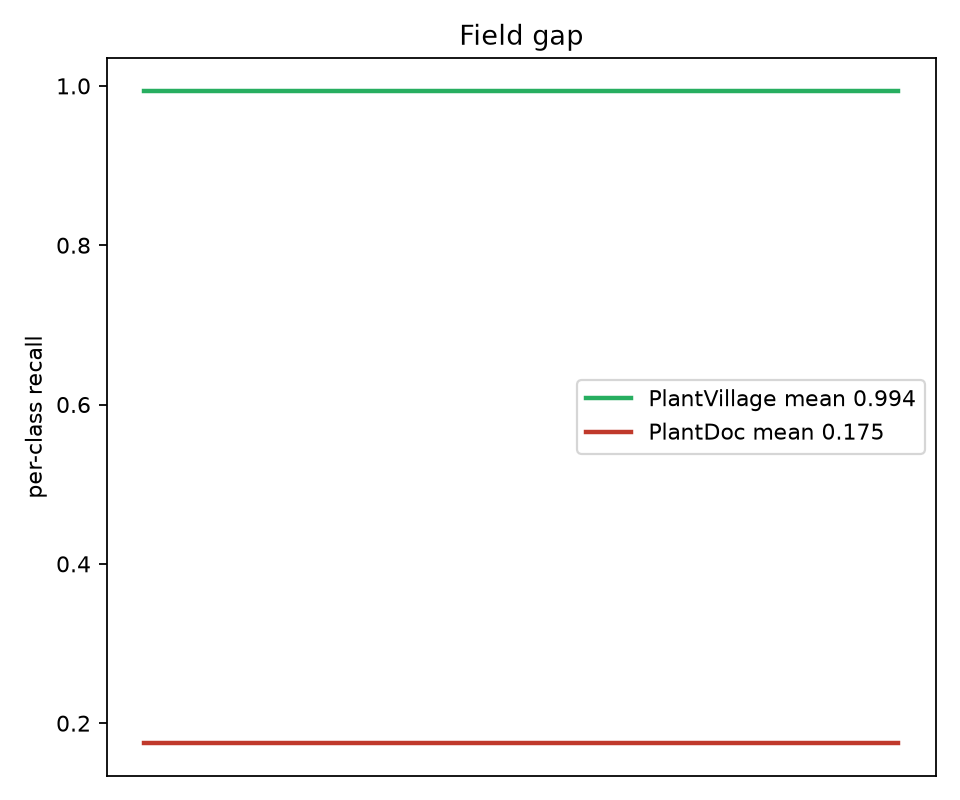
\includegraphics[width=0.92\textwidth]{fig_field_gap.png}
\caption{Curated and field performance for each architecture. Intervals are
bootstrap intervals over the field test set; the curated bars are near the top of
the scale and the field bars are near the bottom, which is the whole finding.}
\label{fig:gap}
\end{figure}

\subsection{Verdict}

H1 is confirmed. The drop is 81.0 points of macro-F1, it replicates across five
seeds, and the interval on the field estimate does not approach the curated figure.

\section{H2: what the decision depends on}

\subsection{Background neutralisation}

Replacing the background with a constant grey patch drops accuracy from 0.9975 to
0.4325 on validation images, a cost of 56.5 points. The background is carrying
information the model needs.

That measurement does not establish what the model is looking at, because a
perturbation that destroys accuracy could do so by making images unlike anything in
training. An intervention that swaps content rather than erasing it answers the
question directly.

\subsection{Swap test}

Each of 298 validation images received a donor from a different class twice.

\begin{table}[H]
\centering
\caption{What moves the prediction, on 298 PlantVillage validation images}
\label{tab:swap}
\tabfont
\begin{tabularx}{\textwidth}{@{}lrrY@{}}
\toprule
\textbf{Measurement} & \textbf{Value} & \textbf{95\,\% interval} & \\
\midrule
Chance adoption, 1 in 38 & 0.0263 & --- & \\
Same-class control, flip rate & 0.0436 & 0.023--0.067 & the edit alone \\
Leaf swap adoption & \textbf{0.5034} & 0.446--0.557 & \\
Background swap adoption & \textbf{0.2181} & 0.171--0.268 & \\
Background minus leaf & $-0.2852$ & $-0.362$ to $-0.205$ & \\
\bottomrule
\end{tabularx}
\end{table}

The control is the load-bearing number. A same-class donor changes the answer 4.4\,\%
of the time, so the compositing itself is not disruptive. Against that floor,
swapping the leaf moves the prediction on half the images, and swapping the
background moves it on one in five, which is eight times chance.

\begin{figure}[H]
\centering
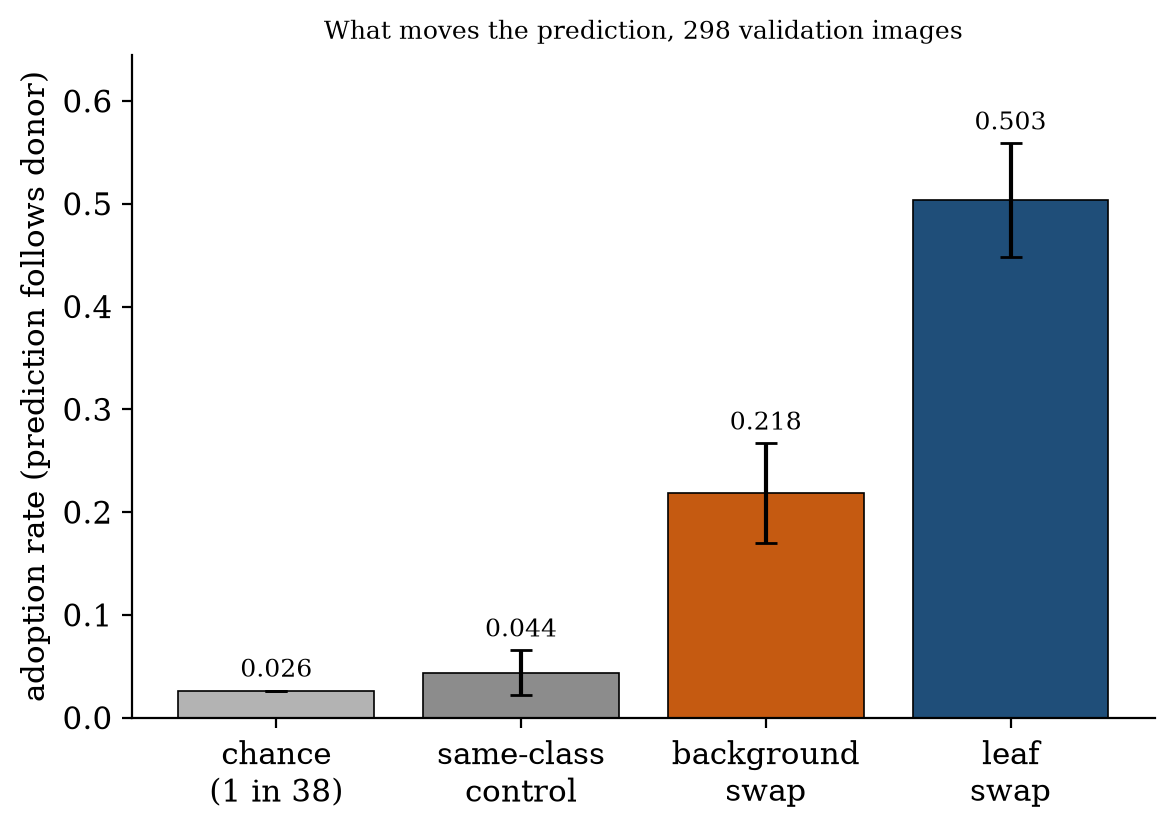
\includegraphics[width=0.86\textwidth]{fig_swap.png}
\caption{Adoption rates from the swap test. Error bars are 95\,\% bootstrap
intervals. The control bar measures how often the edit alone changes the answer, so
everything above it is attributable to the swapped content.}
\label{fig:swap}
\end{figure}

\subsection{Verdict}

H2 is partially supported, and the part matters. The strong form, that the model
reads the scene instead of the plant, is contradicted: the leaf moves the prediction
more than twice as often as the background, and the interval on the difference
excludes zero. The weak form holds: background content can steer the prediction one
time in five, and removing it costs 56.5 points.

The mechanism is joint use of leaf and scene with the leaf carrying more of the
decision. This is a less dramatic finding than the shortcut story and it is the one
the data supports.

\section{H3: background augmentation does not close the gap}

The mechanism result makes a prediction. If the leaf carries most of the signal, then
augmenting the background should recover a portion of the gap and not most of it.
That prediction was recorded before the experiment ran.

Six runs, three seeds per condition, one frozen protocol, differing only in whether
the background-replacement augmentation is enabled.

\begin{table}[H]
\centering
\caption{Paired augmentation experiment, cohort B}
\label{tab:h3}
\tabfont
\begin{tabularx}{\textwidth}{@{}lYYY@{}}
\toprule
\textbf{Condition} & \textbf{In-domain macro-F1} & \textbf{Field macro-F1} & \textbf{Per seed (field)} \\
\midrule
Baseline & 0.9883 & \textbf{0.2232} & 0.2331, 0.2130, 0.2235 \\
Composite & 0.9796 & \textbf{0.2356} & 0.2287, 0.2451, 0.2330 \\
\midrule
Difference & $-0.0087$ & $+0.0124$ & $-0.0044$, $+0.0320$, $+0.0096$ \\
\bottomrule
\end{tabularx}
\end{table}

The 95\,\% interval on the paired difference is $[-3.32, +5.80]$ percentage points,
two of three seeds improved, the sign test gives $p = 0.50$, and the point estimate
recovers 1.6\,\% of the 81-point gap. In-domain accuracy falls by 0.87 points, which
is the expected cost of augmentation and appears in all three pairs.

\subsection{Verdict}

H3 is not supported. There is no detectable effect in the field and a consistent
cost in the lab.

The result is consistent with the mechanism measurement rather than in tension with
it, and that agreement is the substantive finding. Background is used enough to
matter and not enough for randomising it during training to transfer.

\section{H4: a confidence threshold does not rescue the field case}

Calibration is measured on validation, where a threshold may legitimately be chosen.

\begin{table}[H]
\centering
\caption{Reliability and abstention on PlantDoc test}
\label{tab:h4}
\tabfont
\begin{tabularx}{\textwidth}{@{}lrrrrrY@{}}
\toprule
\textbf{Model} & \textbf{Full} & \textbf{95\,\%} & \textbf{90\,\%} & \textbf{80\,\%} & \textbf{50\,\%} & \\
\midrule
ConvNeXt-Tiny & 0.2627 & 0.2679 & 0.2736 & 0.3016 & 0.3644 & \\
ResNet18 & 0.1822 & 0.1875 & 0.1840 & 0.2063 & 0.2458 & \\
EfficientNet-B0 & 0.1737 & 0.1741 & 0.1745 & 0.1852 & 0.2458 & \\
SmallCNN & 0.0678 & 0.0670 & 0.0660 & 0.0582 & 0.0508 & \\
\bottomrule
\end{tabularx}
\end{table}

Calibration error rises from 0.0026 on PlantVillage to 0.5808 on PlantDoc, a factor
of 223. At 90\,\% coverage the reference model gains 0.08 points, from 17.37 to
17.45. Reaching 24.6\,\% requires discarding half the images, and the model is still
wrong three times in four. SmallCNN gets worse when its least confident half is
removed, which means its confidence is anti-correlated with correctness.

\begin{figure}[H]
\centering
\begin{minipage}{0.48\textwidth}\centering
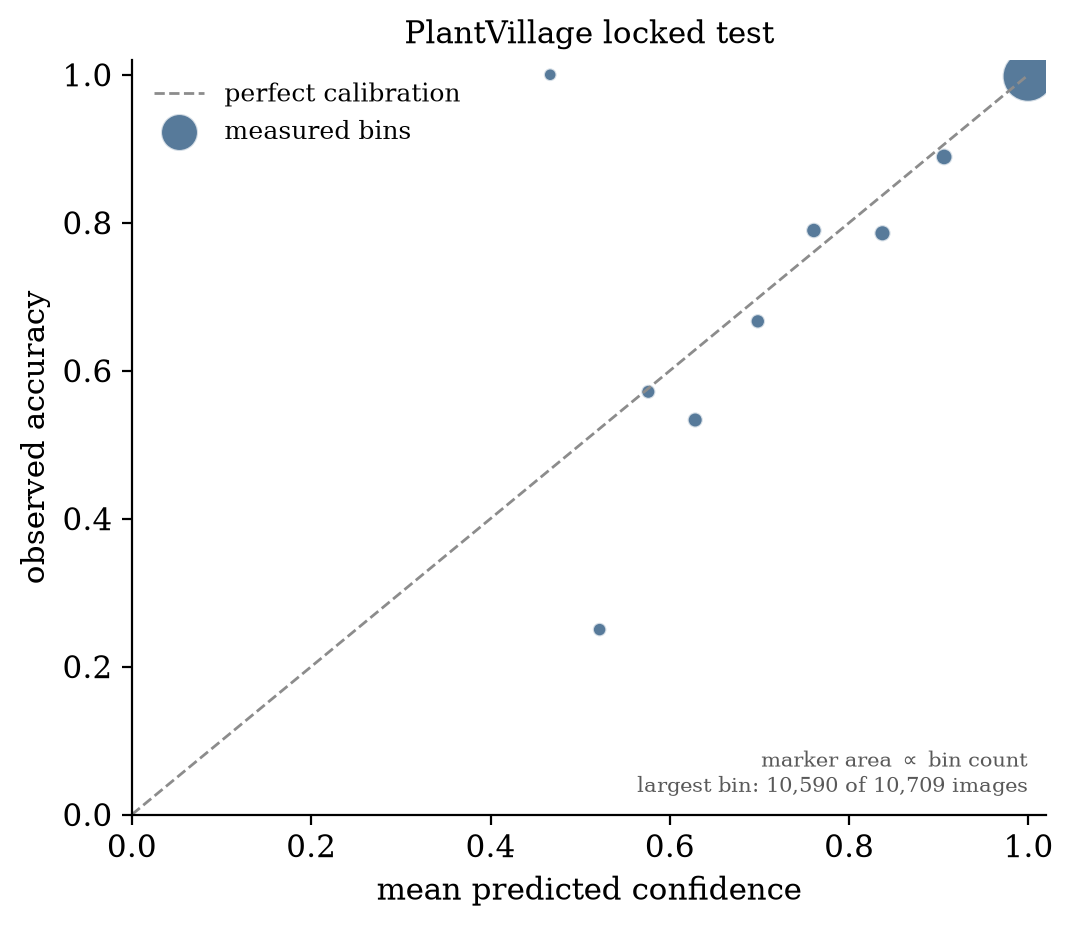
\includegraphics[width=\textwidth]{fig_reliability_test.png}
\end{minipage}\hfill
\begin{minipage}{0.48\textwidth}\centering
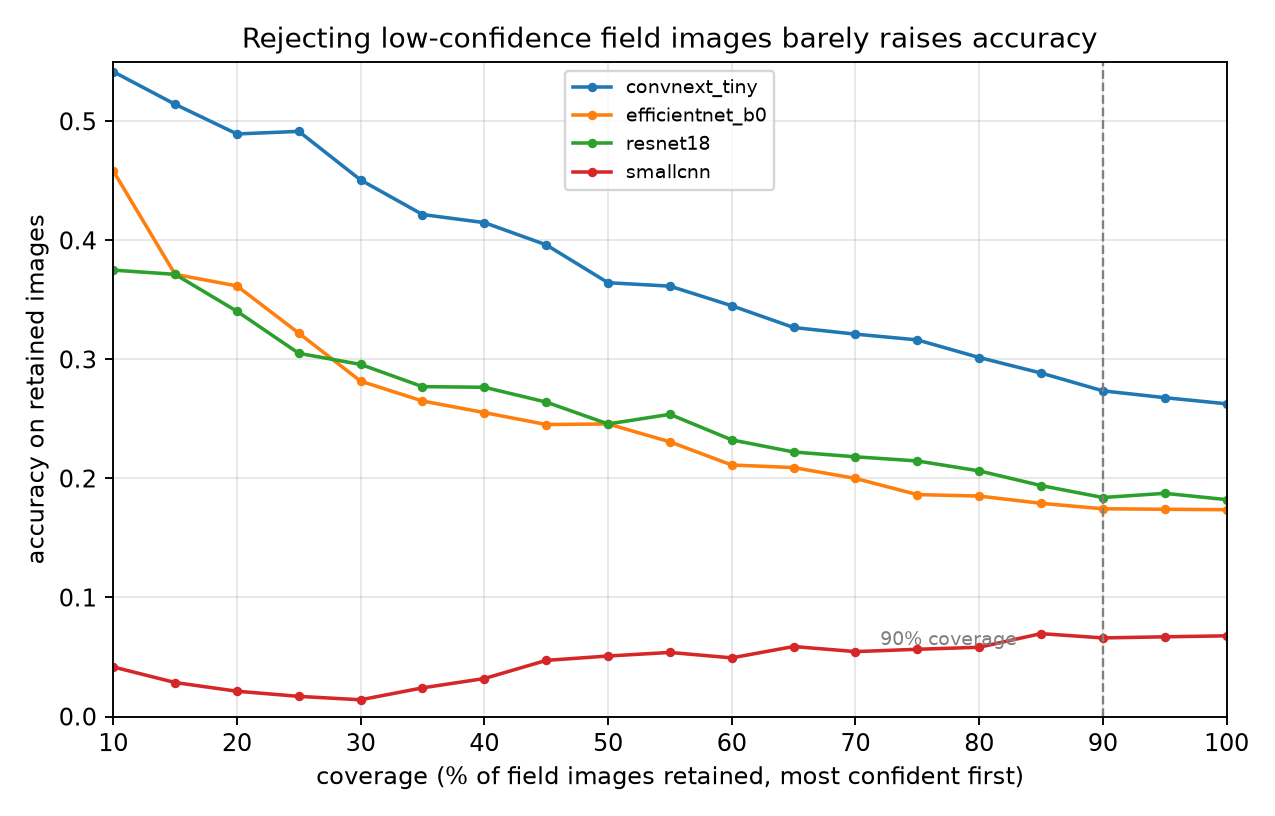
\includegraphics[width=\textwidth]{fig_coverage.png}
\end{minipage}
\caption{Left: reliability on the locked test, where marker area is proportional to
bin count and the single largest bin holds 10,590 of 10,709 images. Right: accuracy
retained as coverage falls, the curve behind Table~\ref{tab:h4}.}
\label{fig:reliability}
\end{figure}

\subsection{Verdict}

H4 is confirmed as a negative finding: the threshold exists and is measured, and it
is not a safety mechanism. Reported failures are genuine failures rather than
flagging failures, and every reported error is a confident error.
